\documentclass{article}

\usepackage[a4paper]{geometry}
\usepackage{amsmath}
\usepackage{amssymb}
\usepackage{amsfonts}
\usepackage{amsthm}
\usepackage{varwidth}
\usepackage{hyperref}
\usepackage{tikz}
\usepackage{tikz-cd}
\usepackage{gensymb}
\usepackage{mathtools}

\usepackage{pgfplots}
\pgfplotsset{compat=1.15}
\usepackage{mathrsfs}
\usetikzlibrary{arrows}
\usetikzlibrary{math}

\newtheorem{lem}{Lemma}
% https://tex.stackexchange.com/a/118217
\DeclarePairedDelimiter\ceil{\lceil}{\rceil}
\DeclarePairedDelimiter\floor{\lfloor}{\rfloor}

\title{POTD 2132}
\author{}
\date{}

\begin{document}

\maketitle

I do not know what I am doing! \\

Let \(f : \mathbb{R} \rightarrow \mathbb{R}\) be a bijective function. Does there always exist an infinite number of functions \(g : \mathbb{R} \rightarrow \mathbb{R}\) such that \(f(g(x)) = g(f(x))\)? \\

Depending on the conditions of \(f\), we can \emph{almost directly} construct an infinity of \(g\). In fact, here we can construct amounts of \(g\) at least as \(\left|\mathbb{R}^{\mathbb{R}}\right|\); how many \(\mathbb{R} \rightarrow \mathbb{R}\) there are generally.

Regard \(\mathbb{R}\) as a digraph where the edges are \((a, f(a))\).

First, let's split up \(\mathbb{R}\) into groups of ``loops''. Construct an equivalence relation \(\sim_f\) on \(\mathbb{R}\) as follows:

\[a \sim_f b := \exists n \in \mathbb{Z} \quad a = f^n(b)\]

that is, \(b\) is ``reachable'' from \(a\) after a number of applications of \(f\) or its inverse. (One can diligently prove that this relation is reflexive, symmetric, and transitive.) \\

Notice that we can characterize every equivalence class in \(\mathbb{R}/\sim_f\) with its number of elements, that is, finitely many or infinitely many (doesn't loop; with the size of \(\mathbb{Z}\)).

For every \emph{finite} equivalence class \(A : \mathbb{R}/\sim_f\), we can pick out an element \(a \in A\) and characterize every element of \(A\) with the minimum positive number of steps to be reached from \(a\). In turn, we form a cyclic graph out of the elements of \(A\):
\[\begin{split}
A \cong C_{|A|} \text{ by } &T_A := x \in A \mapsto \min_{n \in \mathbb{Z}} f^n(a) = x \\
                \text{ and } &T_A^{-1} = n \in C_{|A|} \mapsto f^n(a)
\end{split}\]

call this characteristic \(T\).

For \emph{infinite} equivalence classes \(A : \mathbb{R}/\sim_f\) we can characterize its elements with \(\mathbb{Z}\) instead similarly. (A furious reader may work out the precise equivalence quite hastily.)

\begin{figure}
	\begin{center}
		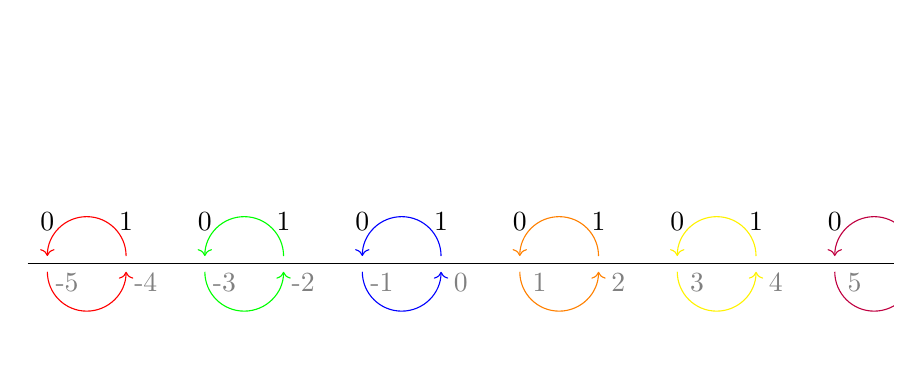
\begin{tikzpicture}
			\clip (-5.5, -1) rectangle (5.5, 3);
			\draw (-5.5,0) -- (5.5,0);
			\foreach \i in {-5,...,5} {
				\draw[below, gray] (\i,0) node {\i};
			}
			\foreach \i/\color in {-5/red,-3/green,-1/blue,1/orange,3/yellow,5/purple} {
				\draw[color=\color, ->] (\i+0.75,0.1)  arc [start angle=0, end angle=180, radius=0.5];
				\draw[color=\color, ->] (\i-0.25,-0.1) arc [start angle=180, end angle=360, radius=0.5];
				\draw[above] (\i+0.75,0.3) node {1};
				\draw[above] (\i-0.25,0.3) node {0};
			}
		\end{tikzpicture}
	\end{center}
	\caption{For the confused reader, here's some of the finite cases where}
	\[f := x \mapsto \begin{cases}x+1 &\text{if } \floor{x} \text{is odd} \\ x-1 &\text{otherwise}\end{cases}\]
\end{figure}

\begin{figure}
	\begin{center}
		\begin{tikzpicture}
			\clip (-5.5, -1) rectangle (5.5, 3);
			\draw (-5.5,0) -- (5.5,0);
			\foreach \i in {-5,...,5} {
				\draw[below, gray] (\i,0) node {\i};
			}
			\foreach \i [evaluate=\i as \n using 3*2^(-\i)] in {-1,...,3} {
				\draw [->] (\n,0) arc [start angle=0, end angle=180, radius=\n/4];
				\draw[below] (\n,-0.3) node {\i};
			}
		\end{tikzpicture}
	\end{center}
	\caption{For the confused reader, here's one of the infinite cases where \(f := x \mapsto \frac{x}{2}\).}
\end{figure}

\newpage

Let us begin constructing \(g\).
We can collect all equivalence classes (as subgraphs) in terms of their size. Let
\begin{align*}
	X_n &:= \left\{A : \mathbb{R}/\sim_f \mid |A| = n\right\} \text{ for } n \in \mathbb{N^+} \\
	X_{\mathbb{Z}} &:= \left\{A : \mathbb{R}/\sim_f \mid A \text{ is (countably) infinitely large}\right\}
\end{align*}
For a fixed \(n \in \mathbb{N}^+ \cup \{\mathbb{Z}\}\), we can see what happens for the canonical graph isomorphism \(h : A \rightarrow B\) for any \(A, B \in X_n\), and with regarding \(h\) also as a digraph/relation,

\begin{align*}
	\forall a \in A \quad h(f(a)) &= h(T_A^{-1}(T_A(f(a))))  \\
							   &= T_B^{-1}(T_A(f(a))) \\
							   &= T_B^{-1}(T_A(a) + 1) \\
							   &= f(T_B^{-1}(T_A(a))) \\
							   &= f(h(a))
\end{align*}

and this is what we exactly needed for the original problem.

\begin{figure}
	% https://q.uiver.app/#q=WzAsMTQsWzEsMCwiXFxidWxsZXQiXSxbMCwxLCJcXGJ1bGxldCJdLFsyLDEsIlxcYnVsbGV0Il0sWzEsMiwiXFxidWxsZXQiXSxbMCwzLCJcXGJ1bGxldCJdLFsyLDMsIlxcYnVsbGV0Il0sWzQsMCwiXFxidWxsZXQiXSxbNCwxLCJcXGJ1bGxldCJdLFs0LDIsIlxcYnVsbGV0Il0sWzQsMywiXFxidWxsZXQiXSxbNSwwLCJcXGJ1bGxldCJdLFs1LDEsIlxcYnVsbGV0Il0sWzUsMiwiXFxidWxsZXQiXSxbNSwzLCJcXGJ1bGxldCJdLFswLDIsImYiLDAseyJzdHlsZSI6eyJ0YWlsIjp7Im5hbWUiOiJtYXBzIHRvIn19fV0sWzIsMSwiZiIsMCx7InN0eWxlIjp7InRhaWwiOnsibmFtZSI6Im1hcHMgdG8ifX19XSxbMSwwLCJmIiwwLHsic3R5bGUiOnsidGFpbCI6eyJuYW1lIjoibWFwcyB0byJ9fX1dLFszLDUsImYiLDAseyJzdHlsZSI6eyJ0YWlsIjp7Im5hbWUiOiJtYXBzIHRvIn19fV0sWzUsNCwiZiIsMCx7InN0eWxlIjp7InRhaWwiOnsibmFtZSI6Im1hcHMgdG8ifX19XSxbNCwzLCJmIiwwLHsic3R5bGUiOnsidGFpbCI6eyJuYW1lIjoibWFwcyB0byJ9fX1dLFsxLDQsImgiLDIseyJzdHlsZSI6eyJ0YWlsIjp7Im5hbWUiOiJtYXBzIHRvIn19fV0sWzIsNSwiaCIsMCx7InN0eWxlIjp7InRhaWwiOnsibmFtZSI6Im1hcHMgdG8ifX19XSxbMCwzLCIiLDEseyJzdHlsZSI6eyJ0YWlsIjp7Im5hbWUiOiJtYXBzIHRvIn19fV0sWzYsNywiZiIsMCx7InN0eWxlIjp7InRhaWwiOnsibmFtZSI6Im1hcHMgdG8ifX19XSxbNyw4LCJmIiwwLHsic3R5bGUiOnsidGFpbCI6eyJuYW1lIjoibWFwcyB0byJ9fX1dLFs4LDksImYiLDAseyJzdHlsZSI6eyJ0YWlsIjp7Im5hbWUiOiJtYXBzIHRvIn19fV0sWzEwLDExLCJmIiwwLHsic3R5bGUiOnsidGFpbCI6eyJuYW1lIjoibWFwcyB0byJ9fX1dLFsxMSwxMiwiZiIsMCx7InN0eWxlIjp7InRhaWwiOnsibmFtZSI6Im1hcHMgdG8ifX19XSxbMTIsMTMsImYiLDAseyJzdHlsZSI6eyJ0YWlsIjp7Im5hbWUiOiJtYXBzIHRvIn19fV0sWzYsMTAsImgiLDEseyJzdHlsZSI6eyJ0YWlsIjp7Im5hbWUiOiJtYXBzIHRvIn19fV0sWzcsMTEsImgiLDEseyJzdHlsZSI6eyJ0YWlsIjp7Im5hbWUiOiJtYXBzIHRvIn19fV0sWzgsMTIsIiBoIiwxLHsic3R5bGUiOnsidGFpbCI6eyJuYW1lIjoibWFwcyB0byJ9fX1dLFs5LDEzLCJoIiwxLHsic3R5bGUiOnsidGFpbCI6eyJuYW1lIjoibWFwcyB0byJ9fX1dXQ==
\[\begin{tikzcd}
	& \bullet &&& \bullet & \bullet \\
	\bullet && \bullet && \bullet & \bullet \\
	& \bullet &&& \bullet & \bullet \\
	\bullet && \bullet && \bullet & \bullet
	\arrow["f", maps to, from=1-2, to=2-3]
	\arrow[maps to, from=1-2, to=3-2]
	\arrow["h"{description}, maps to, from=1-5, to=1-6]
	\arrow["f", maps to, from=1-5, to=2-5]
	\arrow["f", maps to, from=1-6, to=2-6]
	\arrow["f", maps to, from=2-1, to=1-2]
	\arrow["h"', maps to, from=2-1, to=4-1]
	\arrow["f", maps to, from=2-3, to=2-1]
	\arrow["h", maps to, from=2-3, to=4-3]
	\arrow["h"{description}, maps to, from=2-5, to=2-6]
	\arrow["f", maps to, from=2-5, to=3-5]
	\arrow["f", maps to, from=2-6, to=3-6]
	\arrow["f", maps to, from=3-2, to=4-3]
	\arrow["{ h}"{description}, maps to, from=3-5, to=3-6]
	\arrow["f", maps to, from=3-5, to=4-5]
	\arrow["f", maps to, from=3-6, to=4-6]
	\arrow["f", maps to, from=4-1, to=3-2]
	\arrow["f", maps to, from=4-3, to=4-1]
	\arrow["h"{description}, maps to, from=4-5, to=4-6]
\end{tikzcd}\]
	\caption{Diagrams for the confused. Left one is for finite cycle variant, right for the infinite variant.}
\end{figure}

This is what we want for the original problem.

Then we can assign, through the Axiom of Choice:
\begin{enumerate}
\item for any \(n \in \mathbb{N}^+ \cup \{\mathbb{Z}\}\), a function \(X_n \rightarrow X_n\) \\
\item for any \(A \in X_n\), an object \(a \in A\) \\
\end{enumerate}
We must have at least one \(X_n\) to be at least \(|\mathbb{R}|\) in size (otherwise the total \(\bigcup_{n} X_n\) will have a cardinality less than \(\mathbb{R}\))
therefore the number of constructible \(g\) must be at least the number of functions \(X_n \rightarrow X_n\) in size, which is at least the cardinality \(\left|\mathbb{R}^\mathbb{R}\right|\). \(\Box\)

\end{document}